%  LaTeX support: latex@mdpi.com 
%  For support, please attach all files needed for compiling as well as the log file, and specify your operating system, LaTeX version, and LaTeX editor.

%=================================================================
\documentclass[sustainability,article,submit,pdftex,moreauthors]{Definitions/mdpi} 

%--------------------
% Class Options:
%--------------------
%----------
% journal
%----------
% Choose between the following MDPI journals:
% acoustics, actuators, addictions, admsci, adolescents, aerobiology, aerospace, agriculture, agriengineering, agrochemicals, agronomy, ai, air, algorithms, allergies, alloys, analytica, analytics, anatomia, animals, antibiotics, antibodies, antioxidants, applbiosci, appliedchem, appliedmath, applmech, applmicrobiol, applnano, applsci, aquacj, architecture, arm, arthropoda, arts, asc, asi, astronomy, atmosphere, atoms, audiolres, automation, axioms, bacteria, batteries, bdcc, behavsci, beverages, biochem, bioengineering, biologics, biology, biomass, biomechanics, biomed, biomedicines, biomedinformatics, biomimetics, biomolecules, biophysica, biosensors, biotech, birds, bloods, blsf, brainsci, breath, buildings, businesses, cancers, carbon, cardiogenetics, catalysts, cells, ceramics, challenges, chemengineering, chemistry, chemosensors, chemproc, children, chips, cimb, civileng, cleantechnol, climate, clinpract, clockssleep, cmd, coasts, coatings, colloids, colorants, commodities, compounds, computation, computers, condensedmatter, conservation, constrmater, cosmetics, covid, crops, cryptography, crystals, csmf, ctn, curroncol, cyber, dairy, data, ddc, dentistry, dermato, dermatopathology, designs, devices, diabetology, diagnostics, dietetics, digital, disabilities, diseases, diversity, dna, drones, dynamics, earth, ebj, ecologies, econometrics, economies, education, ejihpe, electricity, electrochem, electronicmat, electronics, encyclopedia, endocrines, energies, eng, engproc, entomology, entropy, environments, environsciproc, epidemiologia, epigenomes, est, fermentation, fibers, fintech, fire, fishes, fluids, foods, forecasting, forensicsci, forests, foundations, fractalfract, fuels, future, futureinternet, futurepharmacol, futurephys, futuretransp, galaxies, games, gases, gastroent, gastrointestdisord, gels, genealogy, genes, geographies, geohazards, geomatics, geosciences, geotechnics, geriatrics, grasses, gucdd, hazardousmatters, healthcare, hearts, hemato, hematolrep, heritage, higheredu, highthroughput, histories, horticulturae, hospitals, humanities, humans, hydrobiology, hydrogen, hydrology, hygiene, idr, ijerph, ijfs, ijgi, ijms, ijns, ijpb, ijtm, ijtpp, ime, immuno, informatics, information, infrastructures, inorganics, insects, instruments, inventions, iot, j, jal, jcdd, jcm, jcp, jcs, jcto, jdb, jeta, jfb, jfmk, jimaging, jintelligence, jlpea, jmmp, jmp, jmse, jne, jnt, jof, joitmc, jor, journalmedia, jox, jpm, jrfm, jsan, jtaer, jvd, jzbg, kidneydial, kinasesphosphatases, knowledge, land, languages, laws, life, liquids, literature, livers, logics, logistics, lubricants, lymphatics, machines, macromol, magnetism, magnetochemistry, make, marinedrugs, materials, materproc, mathematics, mca, measurements, medicina, medicines, medsci, membranes, merits, metabolites, metals, meteorology, methane, metrology, micro, microarrays, microbiolres, micromachines, microorganisms, microplastics, minerals, mining, modelling, molbank, molecules, mps, msf, mti, muscles, nanoenergyadv, nanomanufacturing,\gdef\@continuouspages{yes}} nanomaterials, ncrna, ndt, network, neuroglia, neurolint, neurosci, nitrogen, notspecified, %%nri, nursrep, nutraceuticals, nutrients, obesities, oceans, ohbm, onco, %oncopathology, optics, oral, organics, organoids, osteology, oxygen, parasites, parasitologia, particles, pathogens, pathophysiology, pediatrrep, pharmaceuticals, pharmaceutics, pharmacoepidemiology,\gdef\@ISSN{2813-0618}\gdef\@continuous pharmacy, philosophies, photochem, photonics, phycology, physchem, physics, physiologia, plants, plasma, platforms, pollutants, polymers, polysaccharides, poultry, powders, preprints, proceedings, processes, prosthesis, proteomes, psf, psych, psychiatryint, psychoactives, publications, quantumrep, quaternary, qubs, radiation, reactions, receptors, recycling, regeneration, religions, remotesensing, reports, reprodmed, resources, rheumato, risks, robotics, ruminants, safety, sci, scipharm, sclerosis, seeds, sensors, separations, sexes, signals, sinusitis, skins, smartcities, sna, societies, socsci, software, soilsystems, solar, solids, spectroscj, sports, standards, stats, std, stresses, surfaces, surgeries, suschem, sustainability, symmetry, synbio, systems, targets, taxonomy, technologies, telecom, test, textiles, thalassrep, thermo, tomography, tourismhosp, toxics, toxins, transplantology, transportation, traumacare, traumas, tropicalmed, universe, urbansci, uro, vaccines, vehicles, venereology, vetsci, vibration, virtualworlds, viruses, vision, waste, water, wem, wevj, wind, women, world, youth, zoonoticdis 
% For posting an early version of this manuscript as a preprint, you may use "preprints" as the journal. Changing "submit" to "accept" before posting will remove line numbers.

%---------
% article
%---------
% The default type of manuscript is "article", but can be replaced by: 
% abstract, addendum, article, book, bookreview, briefreport, casereport, comment, commentary, communication, conferenceproceedings, correction, conferencereport, entry, expressionofconcern, extendedabstract, datadescriptor, editorial, essay, erratum, hypothesis, interestingimage, obituary, opinion, projectreport, reply, retraction, review, perspective, protocol, shortnote, studyprotocol, systematicreview, supfile, technicalnote, viewpoint, guidelines, registeredreport, tutorial
% supfile = supplementary materials

%----------
% submit
%----------
% The class option "submit" will be changed to "accept" by the Editorial Office when the paper is accepted. This will only make changes to the frontpage (e.g., the logo of the journal will get visible), the headings, and the copyright information. Also, line numbering will be removed. Journal info and pagination for accepted papers will also be assigned by the Editorial Office.

%------------------
% moreauthors
%------------------
% If there is only one author the class option oneauthor should be used. Otherwise use the class option moreauthors.

%---------
% pdftex
%---------
% The option pdftex is for use with pdfLaTeX. Remove "pdftex" for (1) compiling with LaTeX & dvi2pdf (if eps figures are used) or for (2) compiling with XeLaTeX.

%=================================================================
% MDPI internal commands - do not modify
\firstpage{1} 
\makeatletter 
\setcounter{page}{\@firstpage} 
\makeatother
\pubvolume{1}
\issuenum{1}
\articlenumber{0}
\pubyear{2023}
\copyrightyear{2023}
%\externaleditor{Academic Editor: Firstname Lastname}
\datereceived{ } 
\daterevised{ } % Comment out if no revised date
\dateaccepted{ } 
\datepublished{ } 
%\datecorrected{} % For corrected papers: "Corrected: XXX" date in the original paper.
%\dateretracted{} % For corrected papers: "Retracted: XXX" date in the original paper.
\hreflink{https://doi.org/} % If needed use \linebreak
%\doinum{}
%\pdfoutput=1 % Uncommented for upload to arXiv.org

%=================================================================
% Add packages and commands here. The following packages are loaded in our class file: fontenc, inputenc, calc, indentfirst, fancyhdr, graphicx, epstopdf, lastpage, ifthen, float, amsmath, amssymb, lineno, setspace, enumitem, mathpazo, booktabs, titlesec, etoolbox, tabto, xcolor, colortbl, soul, multirow, microtype, tikz, totcount, changepage, attrib, upgreek, array, tabularx, pbox, ragged2e, tocloft, marginnote, marginfix, enotez, amsthm, natbib, hyperref, cleveref, scrextend, url, geometry, newfloat, caption, draftwatermark, seqsplit
% cleveref: load \crefname definitions after \begin{document}

%=================================================================
% Please use the following mathematics environments: Theorem, Lemma, Corollary, Proposition, Characterization, Property, Problem, Example, ExamplesandDefinitions, Hypothesis, Remark, Definition, Notation, Assumption
%% For proofs, please use the proof environment (the amsthm package is loaded by the MDPI class).

%=================================================================
% Full title of the paper (Capitalized)
\Title{A sustainable approach to tourist signage on (historical) trails}

% MDPI internal command: Title for citation in the left column
\TitleCitation{A sustainable approach to tourist signage on historical trails}

% Author Orchid ID: enter ID or remove command
\newcommand{\orcidauthorA}{0000-0000-0000-000X} % Add \orcidA{} behind the author's name
%\newcommand{\orcidauthorB}{0000-0000-0000-000X} % Add \orcidB{} behind the author's name

% Authors, for the paper (add full first names)
\Author{Firstname Lastname $^{1,\dagger,\ddagger}$\orcidA{}, Firstname Lastname $^{2,\ddagger}$ and Firstname Lastname $^{2,}$*}

%\longauthorlist{yes}

% MDPI internal command: Authors, for metadata in PDF
\AuthorNames{Firstname Lastname, Firstname Lastname and Firstname Lastname}

% MDPI internal command: Authors, for citation in the left column
\AuthorCitation{Lastname, F.; Lastname, F.; Lastname, F.}
% If this is a Chicago style journal: Lastname, Firstname, Firstname Lastname, and Firstname Lastname.

% Affiliations / Addresses (Add [1] after \address if there is only one affiliation.)
\address{%
$^{1}$ \quad Affiliation 1; e-mail@e-mail.com\\
$^{2}$ \quad Affiliation 2; e-mail@e-mail.com}

% Contact information of the corresponding author
\corres{Correspondence: e-mail@e-mail.com; Tel.: (optional; include country code; if there are multiple corresponding authors, add author initials) +xx-xxxx-xxx-xxxx (F.L.)}

% Current address and/or shared authorship
\firstnote{Current address: Affiliation 3.} 
\secondnote{These authors contributed equally to this work.}
% The commands \thirdnote{} till \eighthnote{} are available for further notes

%\simplesumm{} % Simple summary

%\conference{} % An extended version of a conference paper

% Abstract (Do not insert blank lines, i.e. \\)
\abstract{
Guiding the visitor to appreciate all aspects of tourist attractions is paramount for building a memorable experience. In the literature, we find many articles exploring the use of sophisticated technologies towards such a goal. The case of wilderness resources exhibits a peculiar aspect, since the presence of human artifacts and the signage, may, in fact, damage the experience, and introduce pollutants as well. In this paper, we consider the case of a natural trail targeted to niche tourism to understand the available options for signage aiming to provide directions, guide the exploration, and warn about dangers. The footprints of the various options are evaluated, and we describe the outcomes of an experimental setup implemented to verify our conclusions' applicability.
}
%\abstract{A single paragraph of about 200 words maximum. For research articles, abstracts should give a pertinent overview of the work. We strongly encourage authors to use the following style of structured abstracts, but without headings: (1) Background: place the question addressed in a broad context and highlight the purpose of the study; (2) Methods: describe briefly the main methods or treatments applied; (3) Results: summarize the article's main findings; (4) Conclusions: indicate the main conclusions or interpretations. The abstract should be an objective representation of the article, it must not contain results which are not presented and substantiated in the main text and should not exaggerate the main conclusions.}

% Keywords
\keyword{keyword 1; keyword 2; keyword 3 (List three to ten pertinent keywords specific to the article; yet reasonably common within the subject discipline.)} 

% The fields PACS, MSC, and JEL may be left empty or commented out if not applicable
%\PACS{J0101}
%\MSC{}
%\JEL{}

%%%%%%%%%%%%%%%%%%%%%%%%%%%%%%%%%%%%%%%%%%
% Only for the journal Diversity
%\LSID{\url{http://}}

%%%%%%%%%%%%%%%%%%%%%%%%%%%%%%%%%%%%%%%%%%
% Only for the journal Applied Sciences
%\featuredapplication{Authors are encouraged to provide a concise description of the specific application or a potential application of the work. This section is not mandatory.}
%%%%%%%%%%%%%%%%%%%%%%%%%%%%%%%%%%%%%%%%%%

%%%%%%%%%%%%%%%%%%%%%%%%%%%%%%%%%%%%%%%%%%
% Only for the journal Data
%\dataset{DOI number or link to the deposited data set if the data set is published separately. If the data set shall be published as a supplement to this paper, this field will be filled by the journal editors. In this case, please submit the data set as a supplement.}
%\datasetlicense{License under which the data set is made available (CC0, CC-BY, CC-BY-SA, CC-BY-NC, etc.)}

%%%%%%%%%%%%%%%%%%%%%%%%%%%%%%%%%%%%%%%%%%
% Only for the journal Toxins
%\keycontribution{The breakthroughs or highlights of the manuscript. Authors can write one or two sentences to describe the most important part of the paper.}

%%%%%%%%%%%%%%%%%%%%%%%%%%%%%%%%%%%%%%%%%%
% Only for the journal Encyclopedia
%\encyclopediadef{For entry manuscripts only: please provide a brief overview of the entry title instead of an abstract.}

%%%%%%%%%%%%%%%%%%%%%%%%%%%%%%%%%%%%%%%%%%
% Only for the journal Advances in Respiratory Medicine
%\addhighlights{yes}
%\renewcommand{\addhighlights}{%

%\noindent This is an obligatory section in “Advances in Respiratory Medicine”, whose goal is to increase the discoverability and readability of the article via search engines and other scholars. Highlights should not be a copy of the abstract, but a simple text allowing the reader to quickly and simplified find out what the article is about and what can be cited from it. Each of these parts should be devoted up to 2~bullet points.\vspace{3pt}\\
%\textbf{What are the main findings?}
% \begin{itemize}[labelsep=2.5mm,topsep=-3pt]
% \item First bullet.
% \item Second bullet.
% \end{itemize}\vspace{3pt}
%\textbf{What is the implication of the main finding?}
% \begin{itemize}[labelsep=2.5mm,topsep=-3pt]
% \item First bullet.
% \item Second bullet.
% \end{itemize}
%}

%%%%%%%%%%%%%%%%%%%%%%%%%%%%%%%%%%%%%%%%%%
\begin{document}

%%%%%%%%%%%%%%%%%%%%%%%%%%%%%%%%%%%%%%%%%%

\section{Introduction}


\subsection{The role of tourist signage}

\section{Tourist signage sustainability}

\subsection{Working hypothesis}

\subsection{Evaluation parameters}

\subsection{Evaluation of sample alternatives}

\section{Application to a concrete use case}

\subsection{Trail selection}

\subsection{Social and political aspects}

\subsection{Signage design}

\subsection{Monitoring results}

\section{Conclusions}


\setcounter{section}{-1} %% Remove this when starting to work on the template.
\section{How to Use this Template}

The template details the sections that can be used in a manuscript. Note that the order and names of article sections may differ from the requirements of the journal (e.g., the positioning of the Materials and Methods section). Please check the instructions on the authors' page of the journal to verify the correct order and names. For any questions, please contact the editorial office of the journal or support@mdpi.com. For LaTeX-related questions please contact latex@mdpi.com.%\endnote{This is an endnote.} % To use endnotes, please un-comment \printendnotes below (before References). Only journal Laws uses \footnote.

% The order of the section titles is different for some journals. Please refer to the "Instructions for Authors” on the journal homepage.

\section{Introduction}

Although an official decision is still pending, there is a sound proposal of naming the time we are living as "anthropocene". Behind such a proposal is the recognition that humans have the potential to significantly alter the environment they live in at a global scale.

The problem behind the above fact is that we humans are not able to understand the consequences of the deployment of such a potential, and not even to keep it under control. Even worse, such capabilities are often used aiming at short-term local effects, ignoring long-term global ones, with the risk of a long-term global deterioration. Such an attitude pervades all activities, starting from the most basic ones like the provision of food and homes, and is frequenly biased by economical profit.

Leisure activities play a relevant role, since they bring profit to niche businesses. This creates a reinforcement effect which follows the negative dynamic seen above: a leisure activity that per se is neutral (e.g. skying) may have a relevant footprint due to induced effects (ski lifts) which reinforces the success of the activity (easier to practice) bringing more investments and impact. Unlike beneficial effects, which is usually well localized, the negative impact has a very wide spectrum encompassing environmental, social and finally economical domains, as discussed by Patthey in \cite{pat08a}.

In an effort to manage such a situation, international agencies promote the "sustainability" keyword as a guideline to the conservation of our habitat. Jeffry Ramsey et al. \cite{ram15a} consider the concept behind the word is "vague and contested but not meaningless" and that it cannot be used without a concrete framework, especially in a normative context. To solve to problem of measuring sustainability, Tom Kuhlman et al. point out a inherent tension in the term between growth and stability. A tension that has been softed by a shift in meaning of the word, which moved from focusing on preservation for an indefinite future to a concept encompassing three "pillars", society, economy and environment, as determinants that need to be protected in the present in view of a future sustainable development. The authors put into relationship man-made and environmental assets, discriminating the two cases in which a loss in the latter may or may not be compensated by an increment of the former, introducinging the terms of {\em weak} and {\em strong} sustainability.

The promotion of the human cultural heritage has its stand in such a complex scenario. As noted by Jorge Otero in \cite{ote22a}, local communities take advantage of heritage promotion: the preservation activity generates social growth, while tourism provides an extra income that may be re-invested in promotion. However, just like in the sky resorts case mentioned above, the risk of compromising the resource itself exists. Such an interplay rises a question of sustainability even for cultural preservation initiatives, two topics that are usually regarded as in synergy. As in the "World Heritage and Sustainable Development" document by Unesco \cite{lab17a} that calls for actions that "harness the potential of World Heritage properties and heritage in general, to contribute to sustainable development".

This paper originates from such a painful contradiction trying to give an answer to the question: is there a way to unlock the potential of a cultural resource limiting the damage to a social, economic and environmental equilibrium?

The question arises in the course of a project funded by the italian ministry of reasearch aiming at the application of cutting edge technologies to the investigation of karst caves that may have been inhabited in the past, from prehistory to today. Among the results expected from the project there is the definition of a strategy to disseminate research results, and allow non-specialists to visit and enjoy the findings, thus contributing to the economy of rural areas that are severely exposed to de-population. A sustainable strategy is even more crucial given that the geological enviroment of interest is notably fragile, as noted by Aleksander Antic\`c et al. in \cite{ant20a}.

This paper provides a concept solution of a specific aspect. The solution is conceptual in that it tries to follow a guideline that takes into account as many side details as possible in a way that can be used in other milieu, but very practical in its unfolding. Given the tighly interconnected nature of the situation, we observe how a vary specific aspect, the touristic signage, exhibits effects on the society, economicy and environment.

\section{Unlocking site potentials through signage}

The signage used to guide and inform the visitor is of paramount importance and must be carefully designed in order to accomplish its functions while following the guidelines of a sustainable approach.

Its functions are twofold
\begin {itemize}
\item an effective signage must guide the tourist across the resort. A map represents a starting point to this end, but not all visitors feel comfortable reading a map. The ideal signage should include visible reference points and explicit actions, like {\em turn right after crossing the stream}. A good example of such a signage is the one used by the Italian Alpine Club (CAI): it consist of a colored stripes marked on tree bark. The marks are placed in such a way that, standing nearby one of them, the hiker is able to see the successive on the trail
\item a sign should explain the reasons of interest of a site. This includes featuring the site where the sign is installed, but also other nearby points of interest that invite the visitor to continue the visit. In this sense, the CAI signal above is not of use. A simple board with a site name may be sufficient only when the site is sufficiently reknown. Otherwise, a more structured message should be used to explain the reasons why the feature is regarded as relevant.
\end{itemize}

In our study we consider a range of solutions that help towards a sustainable support to a sustainable tourism, and specifically to the dynamic provision of information during a visit along a natural trail, not covered by Internet connectivity (a {\em dead zone} using the term used by Pearce and Gretzel \cite{pea12a}). We consider the presence of two stakeholders for the signage itaself \cite{wan22a}: the hosting organization (the {\em host} for short) which implements a signing installation, and the visitor (or {\em user} ) which extracts useful and enjoyable information from signing devices. 

The purpose of such an installation is guiding the {\em user} in a tour that includes urban streets, buildings, natural trails and caves (this latter being the topic of the project giving financial support to our research). The task of the {\em host} organization is to provide the {\em user} with all sorts of information that may guide him across the visit, making it as much profitable and enjoyable as possible.

A traditional approach makes use of physical information boards with graphical or textual contents. Our study starts from finding the issues related with such a solution:

\begin{itemize}
	\item dimensions: the board must be sufficiently large to contain the desired content, taking into account its readability from a distance
	\item installation logistics: depending on the location, the transportation and placement of a plaque may require a basement or other sorts of supports
	\item environmental impact: in order to be effective, the plaque has to be prominent, and this may negatively affect the quality of the site 
	\item accessibility for the visually impaired: the plaque is not useful for visually impaired persons
	\item accessibility for stranger visitors: to limit the size of the plaque, the number of translations must be limited as well
	\item update limits: to update the content, the plaque must be replaced
	\item removal logistics: when the board degrades it must be either removed or replaced, which entails waste disposal together with other issues similar to those found during the installation
\end{itemize}

Such considerations motivate an interest for an alternative way of communication.

\subsection{Technology to minimize intrusion}

We characterize the problem as an instance of {\em weak sustainability}: we do not preclude intervention on the habitat, but the impact of such intervention must be better than that related with traditional signs. To this end we include in our solution tools that are not part of the site but remain with the user.   

During the last decades, we witnessed the diffusion of smartphone devices, and we have no reasons to expect a change in such a trend. Smartphones empower individual communication capabilities, allowing to receive sound, visual and tactile interactions. The relevance of such capabilities for the improvement of a tourist experience have been widely investigated, etiher in urban environments \cite{liu16a} or in a rural milieu \cite{kum20a}. to investigate ways to exploit such tools in our context. Also in this case we start from the limits of such technology, especially in the case of outdoor activities.

One is related with the diffusion of such a technology, which, although widely available, is not equally familiar to everybody. This is related with {\em usability}, with a term borrowed from P. Wan in \cite{wan22a}. The second is that several functions depends on the provision of enabling services: for instance, their networking capability is useless if the device cannot reach an enabling infrastructure. So the {\em applicability limits} of a solution need to be defined.

Starting from the two aspects above we envision the directions towards a successful smartphone-based strategy, keeping in mind the overall sustainability of the approach.

Regarding {\em usability}, the basic recommendation is to keep the operation as simple as possible, within the experience of the majority of users, without requiring the need of installing new applications.

The definition of its {\em applicability limits} is more complex, especially for outdoor activities. In such cases, the provision of a networking infrastructure incurs a severe environmental impact. Consider the installation of antennas to cover a wide area, and the power supply for the radios. 

Circular economy

\subsection{Related works}

The research literature marginally covers the utilization of smartphones for tourist signage purposes.

An exhaustive solution is described by P. Liu in \cite{liu16a}, which provide details for an infrastructure that guides the visitors inside an urban milieu. In that case the presence of a pervasive networking facilities is a cornerstone for the whole architecture, that deeply depends on communication. 

Wan \cite{wan22a} evaluates the quality signage, without making reference to a specific technology, but with many example showing phisical boards, using a formal reference, the Universal Design Principles \cite{udi97a}.

The number of research papers explodes when we extend the range to articles that investigate the impact of smartphones in tourism. The topic {\em smart tourism} topic is very popular, and covered by several review papers that provide a framework to a vast literature.

A relevant research direction covers the social aspects of related with the use of the smartphone. W. Tan \cite{tan17a} covers all aspects of a touristic experience related with the smartphone from the definition of travel destination to assistance during the visit. Much attention is dedicated to the network of connections that is established thanks to the smartphone, which again is considered in the Internet despite the title indicates a nature-based destination, where notably the Internet is not always reachable.

On the other hand, roaming in places not reached by the Internet, or {\em dead zones} using the words of Pearce and Gretzel in \cite{pea12a}, may evoke constrasting feelings, from rewarding to threatening.

More recently, the smartphone has been considered not strictly related with communication. In 2021 A.Slavec et al. investigate the use of cameras \cite{sla21a} while on travel in locations with a relevant cultural heritage in order to sustain its preservation and engage the tourist using location based games, similar to Pokemon Go or geo-caching.

In 2023 V. Rodrigues et al. publish a systematic review of papers considering the interrelationships between tourism and portable digital devices \cite{rod23a}. Although the title evokes a one-way contribution, i.e., the impact of digitalization is assumed to be positive on the quality and the sustainability of touristic offers, in the conclusions the authors reveal awareness for the necessity to address {\em "the preservation of tourism attractions/sites"} and call for for a {\em "a holistic approach ... to support a concept that still lacks conceptual and empirical clarification"}.

In that direction we meet the phenomenon of {\em overtourism}, covered by a significant literature reviewed by Dodds and Butler \cite{dod19a}, which focusses on urban tourism and its social consequences. The impact of {\em overtourism} on resorts that trade on their natural resources is investigated in the case of the Hawaii Islands \cite{lin22a} or CostaRica \cite{mat10a} stressing the imact on the social fabric.

The present paper wants to fill this gap highlighted by Rodriguez, providing a conceptual yet pragmatic approach to a well-defined aspect of tourism support taking into account sustainability by design. Once a range of relevant solutions has been identified, we proceed to the empirical part: a {\em proof of concept} implementation that verifies feasibility of a specific solution.

We stress that this article does not aim now at quantifying user satisfaction or the economic revenue associated with the specific solution. Such a target is outside the scope of our research, and indeed the figures that would represent the success of a strategy deserve further investigation. We aim at isolating an issue, propose a strategy for its solution and implement a proof of concept for it.

% Other papers examine the topic from the point of view of the user satisfaction, with an accent on the accessibility of the contents from impaired users. 

% The use of smartphone is support of a tourist experience is mostly regarded from the point of view of the tourist satisfaction.

% This is the case of 

% Cannot depend on communication

\subsection{A simple, low impact solution}

%Starting from previous experiences documented in the bibliography we explore a few broad categories, to find weaknesses and strengths for each of them.

We aim at designing a strategy for a sustainable and effective smartphone-based signage.

A straightforward approach concentrates on the wireless capabilities of such a device. Given the premise that the Internet is not reachable, the host might provide a local network of low power radios covering the region of interest. Small servers connected to the network might provide specific Web services. The approach requires a modest investment and a marginal environmental impact: for instance, a small device based on the ESP8266 single chip computer (SCC) has a coverage fo tens of meters, and a volume in the order of the $cm^3$. They are able to provide WiFi Access Points as well as Web contents. The ESP8266 has a capacity of 32KB, which are sufficient for an explanatory text and a low resolution image. Other SCCs, like the ESP32, are more powerful but exhibit a higher power consumption. 

The dependency from power supply is a serious limitation of such kind of solution. A radio transmitter is a rather power consuming device, in the range of Watts. Even if operation is intermittent, the operation of the transmitter cannot be guaranteed for long periods and the host organization should consider the installation of a power generator, which contributes to the economical cost and environmental footprint of the device.

For this reason we do not consider a solution based on an ad-hoc network as a valid competitor against traditional board-based design for reasons related with poor sustainability.

An alternative consists in the utilization of passive devices, like Near Field trasmitters. The device is flat with a surface ranging from a credit card to a coin. The receiver must be very close to enable the device to transmits its content. The power needed to operate the radio is drained from the smartphone, so batteries are not needed. The capacity is in the range of the KB, one page on this journal.

The NFC technology is currently very diffused, and reading an NFC tag as text requires the installation of an appropriate application. Once the application is running the operation simply consists in approaching the smartphone to the tag: the tag content is transferred to the smartphone as a chink of text, and can be treated as such. The device can read it aloud to meet the user's inabilities or a translator. For both functions off-line apps exist.

Another solution in the family of passive devices is the QR-code. Such technique does not require radio communication, but uses the smartphone camera to acquire a graphical code that is translated into text. The capacity of a QR-code depends on the number of dots in the code, which in turn depends on the size of the code and the smartphone camera characteristics. We may consider that the capacity of a QR-code roughly equals that of an NFC tag with comparable size but a simpler manufacturing.

% TODO: \usepackage{graphicx} required
\begin{figure}
	\centering
	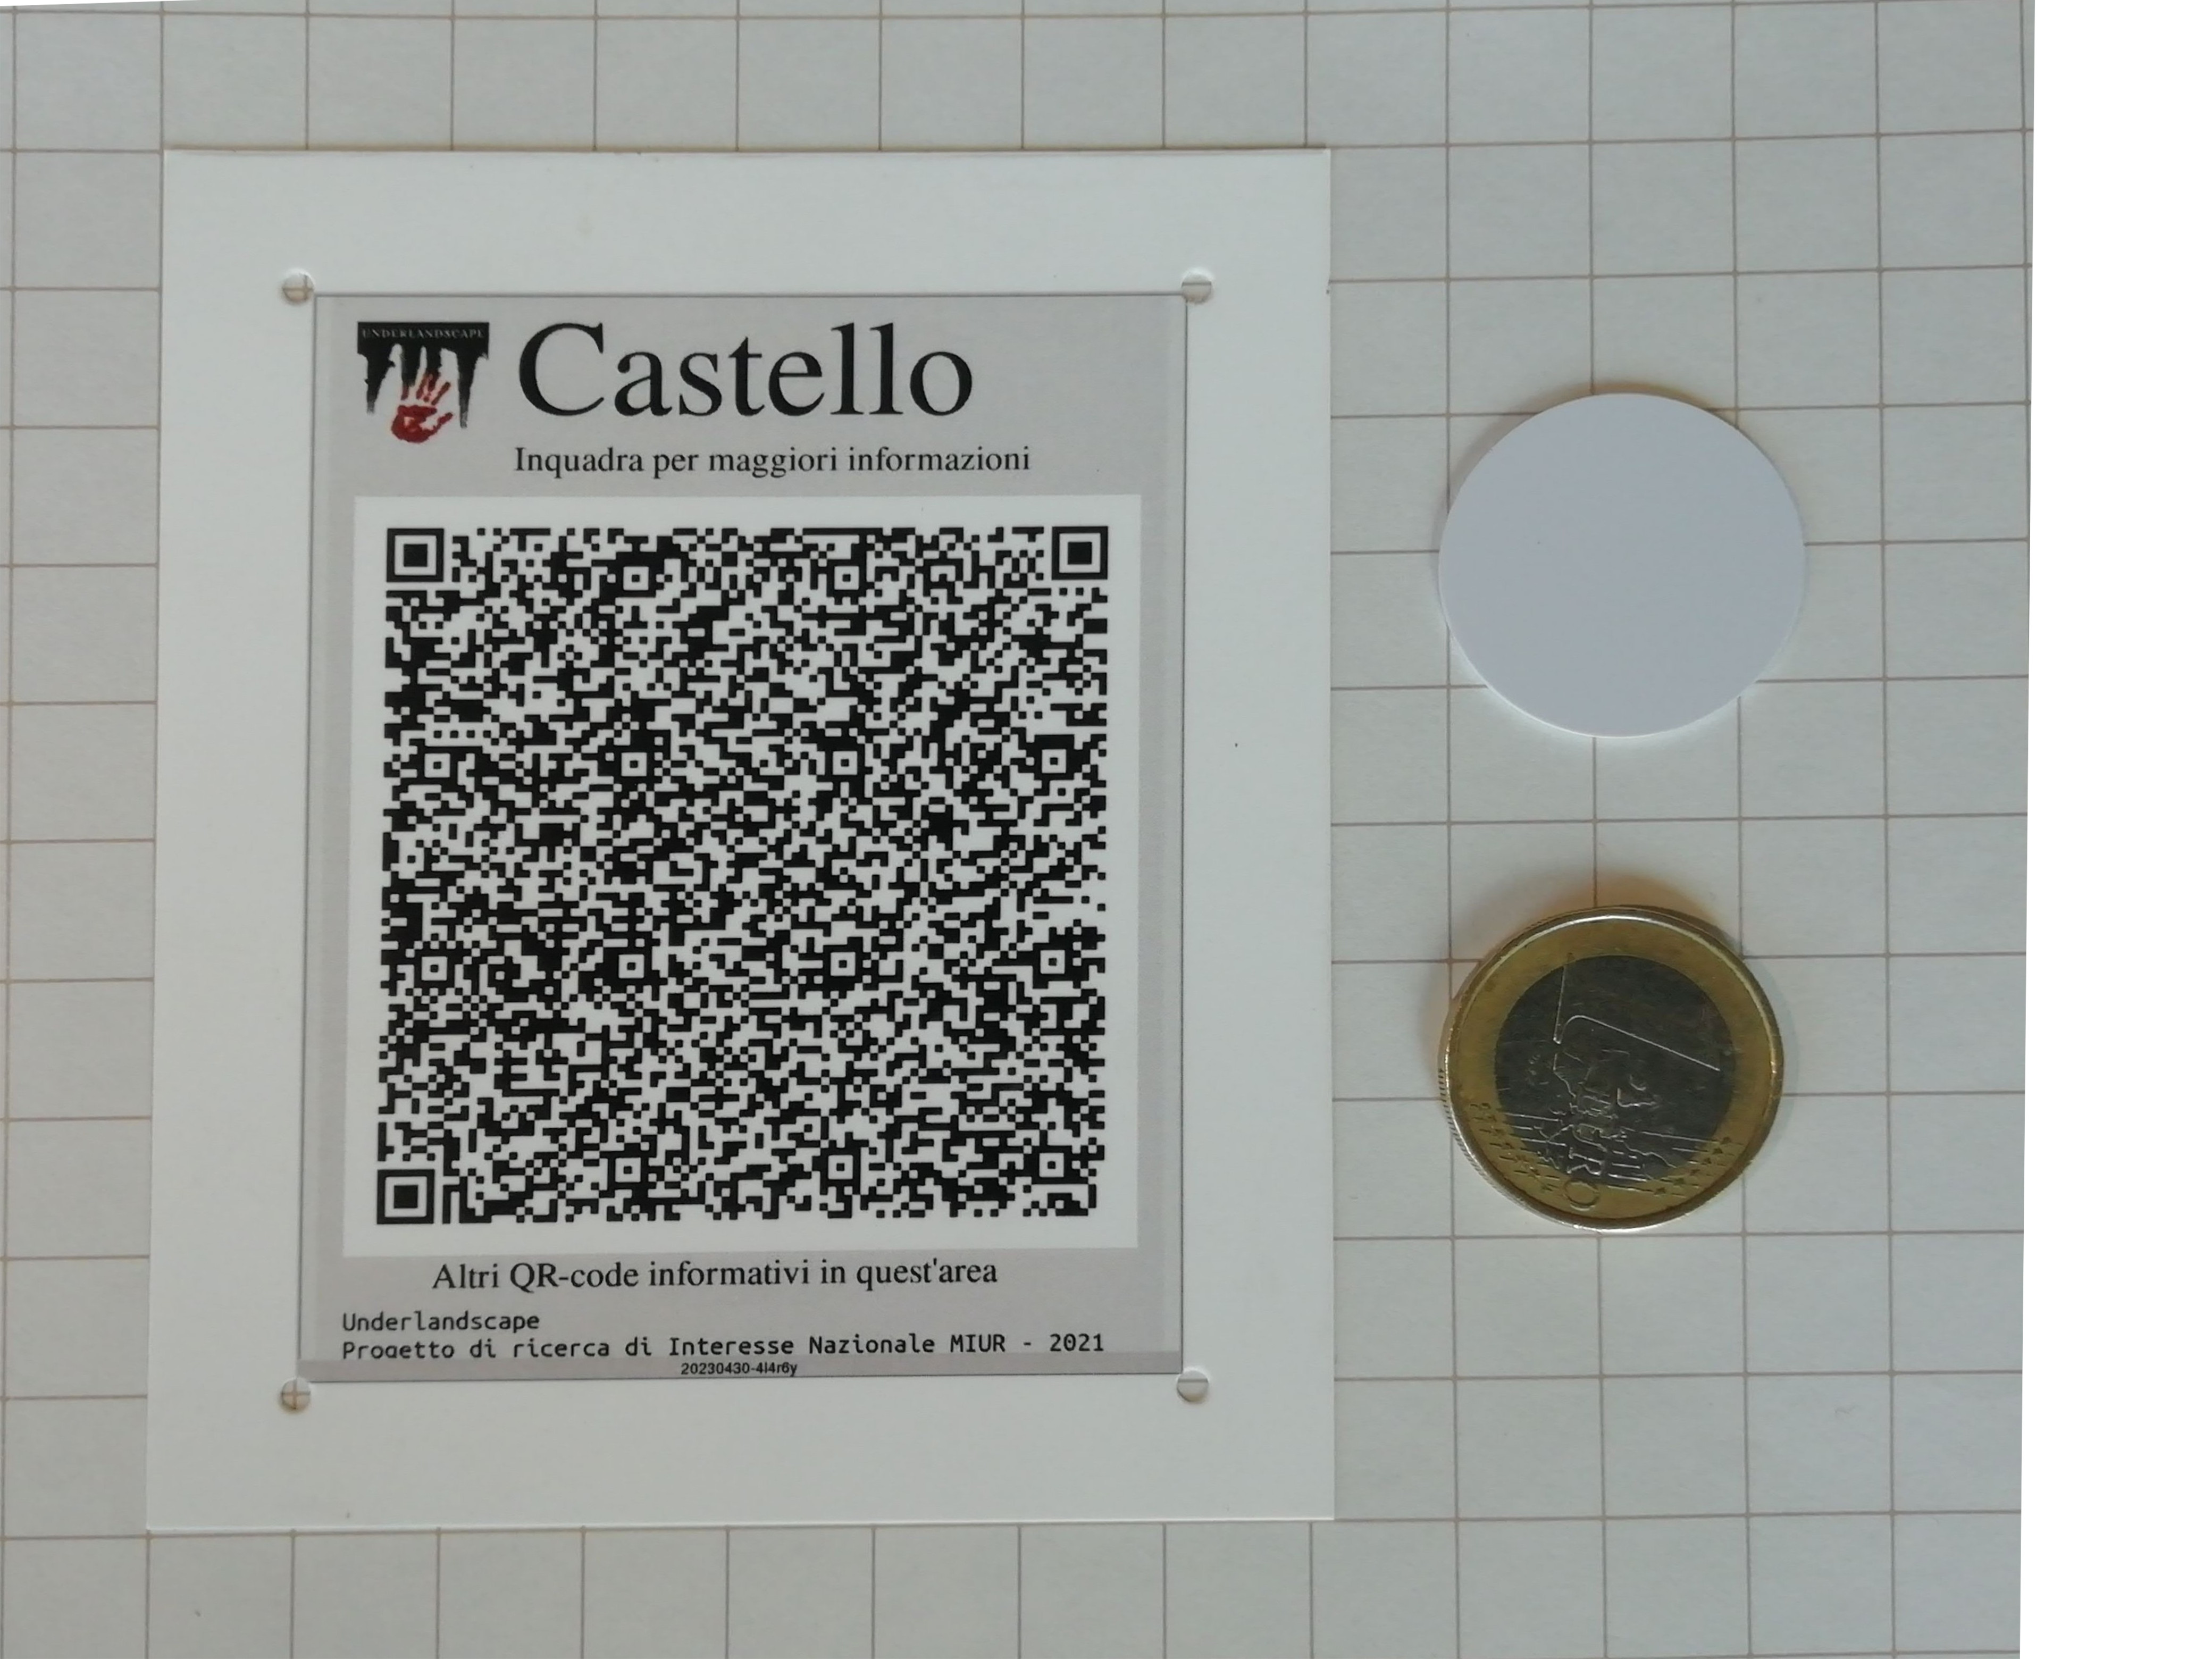
\includegraphics[width=0.9\linewidth]{figure/qr+NFC+coin}
	\caption[Passive devices dimensions]{An NFC coin, a QR-code card used in the project, and a 1 Euro coin by comparison on a paper with a square of 1cm}
	\label{fig:qrnfccoin}
\end{figure}

A preliminary check verifies compliance with the Universal Design Principles \cite{udi97a}:

%\begin{enumerate}
%	\item Equitable Use
%	\item Flexibility in Use
%	\item Simple and Intuitive
%	\item Perceptible Information
%	\item Tolerance for Error
%	\item Low Physical Effort
%	\item Size and Space for Approach and Use
%\end{enumerate}

%The labels are self-descriptive, and we address the reader to the discussion in the referenced document for a more detailed explanation.
%Checking passive devices solutions against the Universal Design principles, we assess their accessibility.

\begin{itemize}
	\item {\em Equitable use} is tighly related to the smartphone technology, which is itself considered a vehicle for equitability,
	\item {\em Flexibility in use} is enabled by the computing capabilities of the device, which allows to listen to the info instead or reading, or translate the information in a different language,
	\item {\em Simple and intuitive use} holds since the operation requires a single application, possibly already installed since useful in many circumstances, and tag reading requires a single touch
	\item{\em Perceptible information} is a critical requirement, which contrasts with the aim of keeping low the environmental intrusion. This point will be further discussed in the section devoted to the implementation
	\item{\em Tolerance for error}: there are no margins to use the device in a way that compromises user safety. The deliberate or accidental release of the passive device into the environment determines a minor pollution
	\item{\em Low physical effort} holds, although the user needs to carry the smartphone
	\item{Size and Space for approach and use} have to be carefully considered. In the case of the NFC the smartphone needs to be nearly in touch with the passive device, while the QR-code must be in line of sight and frameable without effort
\end{itemize}

Such a minimalistic solutions (se figure \ref{fig:qrnfccoin}) compares well compared with other solutions that make use of the user's smartphone. There is a trade-off concerning capacity, but in many circumstances a capacity of 2-300 words is sufficient to convey the description of the site, or provide directions for the the visit. If capacity is not an issue a solution based on NFC or QR-codes exhibits a number of advantages:
\begin{itemize} 
\item does not require any power supply
\item has a limited impact on the landscape
\item is not exposed to theft
\item has a negligible cost
\item is durable
\item produces a limited quantity of waste when disposed
\item the content can be stored by the user's device for successive utilization
\end{itemize}

%It significantly outperforms any active device, except for the capacity, and the NFC compares favorably only when capacity and size are prominent.  

A solution based on the user smartphone associated with passive devices compares favorably with traditional signage boards. Considering the limits of the latter approach listed in table \ref{tab:board}:

%The adoption of passive devices compares favorably with traditional boards, considering the strengths and limits as listed above.

\begin{itemize}
	\item dimensions: a 2-300 characters QR-code has a dimension in the order of 100 $cm^2$
	\item logistics: QR-code board can be installed on any sort of pre-existent or natural support
	\item impact: the board has a minimal interference with the landscape and may easely go un-noticed if not properly advertised
	\item accessibility for the visually impaired: the text can be read aloud
	\item international: the text can be translated
	\item update: the board can be easely replaced when the content becomes obsolete
	\item disposal: the card releases a limited quantity of pollutants related with ink support (paper or plastic)
\end{itemize}
		
%One of the issues the host must resolve is the availability of support for electronic devices. The provisioon of such support has a footprint that ha		
%may be present, but, in the spirit of our investigation, power supply should be address renewable sources, like wind, sunlight and similar.
%One option discriminates the use of an electronic device on the side of the user. 
%In case we assume the user does not have a electronic device with her, the 
%One option is to introduce active electronics: the touristic site administration provides a 
		
There are two relevant trade-offs that the host needs to resolve. One is related with the visibility of the tag. The trade-off is among the  

\section{Materials and Methods}

In our study we have considered a range of solutions that may help towards our goal of a sustainable support to a sustainable tourism, and specifically to the dynamic provision of information during a visit. To this end, the hosting organization (the {\em host} for short) implements a system of devices from which the visitor (or {\em user} ) extracts useful and enjoyable information. 

The purpose of such an installation is to guide the {\em user} in a tour that includes hurban streets, buildings, natural trails and caves (this latter being the topic of the project giving financial support to our research). The task of the host organization is to provide the user with all sorts of information that may guide him across the visit, making it as much profitable and enjoyable as possible.

A traditional approach makes use of physical information boards with graphical or textual contents. Our study starts from finding the issues related with such a solution:

\begin{itemize}
\item dimensions: the board must be sufficiently large to contain the desired content, taking into account its readability from a distance
\item installation logistics: depending on the location, the placement of a plaque may require a basement or other sorts of supports
\item environmental impact: in order to be effective, the plaque is prominent, and this may negatively affect the quality of the site 
\item accessibility for the visually impaired: the plaque is not useful for visually impaired persons
\item accessibility for stranger visitors: to limit the size of the plaque, the number of translations must be limited as well
\item update limits: to update the content, the plaque must be replaced
\item removal logistics: when the board degrades it must be either removed or replaced, which entails waste disposal together with other issues like those found during the installation
\end{itemize}

Such considerations motivate an interest for an alternative way of communication. 

During the last decades we have witnessed the diffusion of smartphone devices, and we have no reasons to expect a change in such a thread. Smartphones empower the communication capabilities of an individual, allowing to receive sound, visual and tatcile interactions. It is therefore straightforward to consider the way to exploit such capabilities in our context. Also in this case we start from the limits of such technology.

Concentrate on outdoor activities

One is related with the diffusion of such a technology, which, although very diffused, is not equally familiar to everybody. The second is that several functions depends on the provision of enabling services: for instance, their networking capability is useless if the device cannot reach an enabling infrastructure.

Starting from the two aspects above we envision the directions towards a successful strategy, keeping in mind the overall sustainability of the approach.

Regarding usability, the basic recommendation is to keep the operation as simple as possible, within the experience of the majority of users, without requiring the need of installing new applications.

The second issue is more complex, especially when considering outdoor activities. In such cases the provision of a networking infrastructure may be impossibile without a severe environmental impact. Consider the installation of antennas to cover a wide area and power supply for the radios. 

Starting from previous experiences documented in the bibliography we explore a few broad categories, to find weaknesses and strengths for each of them.

One strategy concentrates on the wireless capabilities of the smartphone, although avoiding the coverage of the whole region. We consider the implementation of several small servers operating in isolation that provide a few HTML pages. The approach requires a modest investment and a marginal environmental impact: a small device based on the ESP8266 single chip computer has a coverage fo tens of meters, and a volume in the order of the $cm^3$. They operate as WiFi Access Points, so the user has access to the data in the device by joining the AP and browsing the URL. The ESP8266 has a capacity of 32KB, which are sufficient for an explanatory text and a low resolution image.

The dependency from power supply is a serious limitation of such kind of solution. A radio transmitter is a rather power consuming device, in the range of Watts. Even if operation is intermittent, the operation of the transmitter cannot be guaranteed for long periods and the host organizaton should consider the installation of a power generator, which contributes to the economical cost and environmental footprint of the device,

An alternative consists in the utilization of passive devices, like Near Field trasmitters. The device is flat with a surface ranging from a credit card to a coin. The receiver must be very close to enable the device to transmits its content. The power needed to operate the radio is drained from the smartphone, so batteries are not needed. The capacity is in the range of the KB, one page on this journal.

The NFC technology is currently very diffused, and reading an NFC tag as text requires the installation of an appropriate application. Once the application is running the operation simply consists in approaching the smartphone to the tag: the tag content is trasferred to the smartphone as a chink of text, and can be treated as such. The device can read it aloud to meet the user's inabilities or a translator. For both functions off-line apps exist to compensate the lack of network connection.

Another solution in the family of passive devices is the QR-code. Such technique does not require radio communication, but uses the smartphone camera to acquire a graphical code that can be translated into a text. The capacity of a QR-code depends on the number of dots in the code, which in turn depends on the size of the code and the smartphone camera. We may consider that the capacity of a QR-code roughly equals that of an NFC tag with comparable size but a simpler manufacturing.

Such a minimalistic solution compares surprisingly well when compared with other solutions that make use of the user's smartphone. There is a trade-off concerning capacity, but in many circumstances a capacity of 2-300 words are sufficient to convey the description of a site, or provide directions for the the visit. In exchange, the QR-code solution does not require any power supply, is extremely easy to use, has a limited impact on the laandscape, is not exposed to theft, has a negligible cost, is durable and produces a limited quantity of garbage when disposed, is readable at a moderate distance and can be read aloud, translated or stored by the user's device. It significantly outperforms any active device, except for the capacity, and the NFC compares favorably only when capacity and size are prominent.  

The adoption of QR-codes compares favorably with traditional boards, considering the strengths and limits as listed above.

\begin{itemize}
\item dimensions: a 2-300 characters QR-code has the dimensione of a poker card
\item logistics: QR-code board can be installed on any sort of preexisting support
\item impact: the board has a minimal interference with the landscape and may easely go un-noticed if not properly advertised
\item accessibility for the visually impaired: the text can be read aloud
\item international: the text can be translated
\item update: the board can be easely replaced when the content turns obsolete
\item disposal: the card releases a limited quantity of pollutants related with ink support (paper or plastic)
\end{itemize}



One of the issues the host must resolve is the availability of support for electronic devices. The provisioon of such support has a footprint that ha

may be present, but, in the spirit of our investigation, power supply should be address renewable sources, like wind, sunlight and similar.



One option discriminates the use of an electronic device on the side of the user. 

In case we assume the user does not have a electronic device with her, the 
One option is to introduce active electronics: the touristic site administration provides a 


%Materials and Methods should be described with sufficient details to allow others to replicate and build on published results. Please note that publication of your manuscript implicates that you must make all materials, data, computer code, and protocols associated with the publication available to readers. Please disclose at the submission stage any restrictions on the availability of materials or information. New methods and protocols should be described in detail while well-established methods can be briefly described and appropriately cited.

%Research manuscripts reporting large datasets that are deposited in a publicly avail-able database should specify where the data have been deposited and provide the relevant accession numbers. If the accession numbers have not yet been obtained at the time of submission, please state that they will be provided during review. They must be provided prior to publication.

%Interventionary studies involving animals or humans, and other studies require ethical approval must list the authority that provided approval and the corresponding ethical approval code.
%\begin{quote}
%This is an example of a quote.
%\end{quote}

%%%%%%%%%%%%%%%%%%%%%%%%%%%%%%%%%%%%%%%%%%
\section{Results}

This section may be divided by subheadings. It should provide a concise and precise description of the experimental results, their interpretation as well as the experimental conclusions that can be drawn.
\subsection{Subsection}
\subsubsection{Subsubsection}

Bulleted lists look like this:
\begin{itemize}
\item	First bullet;
\item	Second bullet;
\item	Third bullet.
\end{itemize}

Numbered lists can be added as follows:
\begin{enumerate}
\item	First item; 
\item	Second item;
\item	Third item.
\end{enumerate}

The text continues here. 

\subsection{Figures, Tables and Schemes}

All figures and tables should be cited in the main text as Figure~\ref{fig1}, Table~\ref{tab1}, etc.

\begin{figure}[H]

\includegraphics[width=10.5 cm]{Definitions/logo-mdpi}
\caption{This is a figure. Schemes follow the same formatting. If there are multiple panels, they should be listed as: (\textbf{a}) Description of what is contained in the first panel. (\textbf{b}) Description of what is contained in the second panel. Figures should be placed in the main text near to the first time they are cited. A caption on a single line should be centered.\label{fig1}}
\end{figure}   
\unskip

\begin{table}[H] 
\caption{This is a table caption. Tables should be placed in the main text near to the first time they are~cited.\label{tab1}}
\newcolumntype{C}{>{\centering\arraybackslash}X}
\begin{tabularx}{\textwidth}{CCC}
\toprule
\textbf{Title 1}	& \textbf{Title 2}	& \textbf{Title 3}\\
\midrule
Entry 1		& Data			& Data\\
Entry 2		& Data			& Data \textsuperscript{1}\\
\bottomrule
\end{tabularx}
\noindent{\footnotesize{\textsuperscript{1} Tables may have a footer.}}
\end{table}

The text continues here (Figure~\ref{fig2} and Table~\ref{tab2}).

% Example of a figure that spans the whole page width. The same concept works for tables, too.
\begin{figure}[H]
\begin{adjustwidth}{-\extralength}{0cm}
\centering

\includegraphics[width=15.5cm]{Definitions/logo-mdpi}
\end{adjustwidth}
\caption{This is a wide figure.\label{fig2}}
\end{figure}  

\begin{table}[H]
\caption{This is a wide table.\label{tab2}}
	\begin{adjustwidth}{-\extralength}{0cm}
		\newcolumntype{C}{>{\centering\arraybackslash}X}
		\begin{tabularx}{\fulllength}{CCCC}
			\toprule
			\textbf{Title 1}	& \textbf{Title 2}	& \textbf{Title 3}     & \textbf{Title 4}\\
			\midrule
\multirow[m]{3}{*}{Entry 1 *}	& Data			& Data			& Data\\
			  	                   & Data			& Data			& Data\\
			             	      & Data			& Data			& Data\\
                   \midrule
\multirow[m]{3}{*}{Entry 2}    & Data			& Data			& Data\\
			  	                  & Data			& Data			& Data\\
			             	     & Data			& Data			& Data\\
                   \midrule
\multirow[m]{3}{*}{Entry 3}    & Data			& Data			& Data\\
			  	                 & Data			& Data			& Data\\
			             	    & Data			& Data			& Data\\
                  \midrule
\multirow[m]{3}{*}{Entry 4}   & Data			& Data			& Data\\
			  	                 & Data			& Data			& Data\\
			             	    & Data			& Data			& Data\\
			\bottomrule
		\end{tabularx}
	\end{adjustwidth}
	\noindent{\footnotesize{* Tables may have a footer.}}
\end{table}

%\begin{listing}[H]
%\caption{Title of the listing}
%\rule{\columnwidth}{1pt}
%\raggedright Text of the listing. In font size footnotesize, small, or normalsize. Preferred format: left aligned and single spaced. Preferred border format: top border line and bottom border line.
%\rule{\columnwidth}{1pt}
%\end{listing}

Text.

Text.

\subsection{Formatting of Mathematical Components}

This is the example 1 of equation:
\begin{linenomath}
\begin{equation}
a = 1,
\end{equation}
\end{linenomath}
the text following an equation need not be a new paragraph. Please punctuate equations as regular text.
%% If the documentclass option "submit" is chosen, please insert a blank line before and after any math environment (equation and eqnarray environments). This ensures correct linenumbering. The blank line should be removed when the documentclass option is changed to "accept" because the text following an equation should not be a new paragraph.

This is the example 2 of equation:
\begin{adjustwidth}{-\extralength}{0cm}
\begin{equation}
a = b + c + d + e + f + g + h + i + j + k + l + m + n + o + p + q + r + s + t + u + v + w + x + y + z
\end{equation}
\end{adjustwidth}

% Example of a page in landscape format (with table and table footnote).
%\startlandscape
%\begin{table}[H] %% Table in wide page
%\caption{This is a very wide table.\label{tab3}}
%	\begin{tabularx}{\textwidth}{CCCC}
%		\toprule
%		\textbf{Title 1}	& \textbf{Title 2}	& \textbf{Title 3}	& \textbf{Title 4}\\
%		\midrule
%		Entry 1		& Data			& Data			& This cell has some longer content that runs over two lines.\\
%		Entry 2		& Data			& Data			& Data\textsuperscript{1}\\
%		\bottomrule
%	\end{tabularx}
%	\begin{adjustwidth}{+\extralength}{0cm}
%		\noindent\footnotesize{\textsuperscript{1} This is a table footnote.}
%	\end{adjustwidth}
%\end{table}
%\finishlandscape


Please punctuate equations as regular text. Theorem-type environments (including propositions, lemmas, corollaries etc.) can be formatted as follows:
%% Example of a theorem:
\begin{Theorem}
Example text of a theorem.
\end{Theorem}

The text continues here. Proofs must be formatted as follows:

%% Example of a proof:
\begin{proof}[Proof of Theorem 1]
Text of the proof. Note that the phrase ``of Theorem 1'' is optional if it is clear which theorem is being referred to.
\end{proof}
The text continues here.

%%%%%%%%%%%%%%%%%%%%%%%%%%%%%%%%%%%%%%%%%%
\section{Discussion}

Authors should discuss the results and how they can be interpreted from the perspective of previous studies and of the working hypotheses. The findings and their implications should be discussed in the broadest context possible. Future research directions may also be highlighted.

%%%%%%%%%%%%%%%%%%%%%%%%%%%%%%%%%%%%%%%%%%
\section{Conclusions}

This section is not mandatory, but can be added to the manuscript if the discussion is unusually long or complex.

%%%%%%%%%%%%%%%%%%%%%%%%%%%%%%%%%%%%%%%%%%
\section{Patents}

This section is not mandatory, but may be added if there are patents resulting from the work reported in this manuscript.

%%%%%%%%%%%%%%%%%%%%%%%%%%%%%%%%%%%%%%%%%%
\vspace{6pt} 

%%%%%%%%%%%%%%%%%%%%%%%%%%%%%%%%%%%%%%%%%%
%% optional
%\supplementary{The following supporting information can be downloaded at:  \linksupplementary{s1}, Figure S1: title; Table S1: title; Video S1: title.}

% Only for the journal Methods and Protocols:
% If you wish to submit a video article, please do so with any other supplementary material.
% \supplementary{The following supporting information can be downloaded at: \linksupplementary{s1}, Figure S1: title; Table S1: title; Video S1: title. A supporting video article is available at doi: link.}

%%%%%%%%%%%%%%%%%%%%%%%%%%%%%%%%%%%%%%%%%%
\authorcontributions{For research articles with several authors, a short paragraph specifying their individual contributions must be provided. The following statements should be used ``Conceptualization, X.X. and Y.Y.; methodology, X.X.; software, X.X.; validation, X.X., Y.Y. and Z.Z.; formal analysis, X.X.; investigation, X.X.; resources, X.X.; data curation, X.X.; writing---original draft preparation, X.X.; writing---review and editing, X.X.; visualization, X.X.; supervision, X.X.; project administration, X.X.; funding acquisition, Y.Y. All authors have read and agreed to the published version of the manuscript.'', please turn to the  \href{http://img.mdpi.org/data/contributor-role-instruction.pdf}{CRediT taxonomy} for the term explanation. Authorship must be limited to those who have contributed substantially to the work~reported.}

\funding{Please add: ``This research received no external funding'' or ``This research was funded by NAME OF FUNDER grant number XXX.'' and  and ``The APC was funded by XXX''. Check carefully that the details given are accurate and use the standard spelling of funding agency names at \url{https://search.crossref.org/funding}, any errors may affect your future funding.}

\institutionalreview{In this section, you should add the Institutional Review Board Statement and approval number, if relevant to your study. You might choose to exclude this statement if the study did not require ethical approval. Please note that the Editorial Office might ask you for further information. Please add “The study was conducted in accordance with the Declaration of Helsinki, and approved by the Institutional Review Board (or Ethics Committee) of NAME OF INSTITUTE (protocol code XXX and date of approval).” for studies involving humans. OR “The animal study protocol was approved by the Institutional Review Board (or Ethics Committee) of NAME OF INSTITUTE (protocol code XXX and date of approval).” for studies involving animals. OR “Ethical review and approval were waived for this study due to REASON (please provide a detailed justification).” OR “Not applicable” for studies not involving humans or animals.}

\informedconsent{Any research article describing a study involving humans should contain this statement. Please add ``Informed consent was obtained from all subjects involved in the study.'' OR ``Patient consent was waived due to REASON (please provide a detailed justification).'' OR ``Not applicable'' for studies not involving humans. You might also choose to exclude this statement if the study did not involve humans.

Written informed consent for publication must be obtained from participating patients who can be identified (including by the patients themselves). Please state ``Written informed consent has been obtained from the patient(s) to publish this paper'' if applicable.}

\dataavailability{We encourage all authors of articles published in MDPI journals to share their research data. In this section, please provide details regarding where data supporting reported results can be found, including links to publicly archived datasets analyzed or generated during the study. Where no new data were created, or where data is unavailable due to privacy or ethical re-strictions, a statement is still required. Suggested Data Availability Statements are available in section “MDPI Research Data Policies” at \url{https://www.mdpi.com/ethics}.} 

\acknowledgments{In this section you can acknowledge any support given which is not covered by the author contribution or funding sections. This may include administrative and technical support, or donations in kind (e.g., materials used for experiments).}

\conflictsofinterest{Declare conflicts of interest or state ``The authors declare no conflict of interest.'' Authors must identify and declare any personal circumstances or interest that may be perceived as inappropriately influencing the representation or interpretation of reported research results. Any role of the funders in the design of the study; in the collection, analyses or interpretation of data; in the writing of the manuscript; or in the decision to publish the results must be declared in this section. If there is no role, please state ``The funders had no role in the design of the study; in the collection, analyses, or interpretation of data; in the writing of the manuscript; or in the decision to publish the~results''.} 

%%%%%%%%%%%%%%%%%%%%%%%%%%%%%%%%%%%%%%%%%%
%% Optional
\sampleavailability{Samples of the compounds ... are available from the authors.}

%% Only for journal Encyclopedia
%\entrylink{The Link to this entry published on the encyclopedia platform.}

\abbreviations{Abbreviations}{
The following abbreviations are used in this manuscript:\\

\noindent 
\begin{tabular}{@{}ll}
MDPI & Multidisciplinary Digital Publishing Institute\\
DOAJ & Directory of open access journals\\
TLA & Three letter acronym\\
LD & Linear dichroism
\end{tabular}
}

%%%%%%%%%%%%%%%%%%%%%%%%%%%%%%%%%%%%%%%%%%
%% Optional
\appendixtitles{no} % Leave argument "no" if all appendix headings stay EMPTY (then no dot is printed after "Appendix A"). If the appendix sections contain a heading then change the argument to "yes".
\appendixstart
\appendix
\section[\appendixname~\thesection]{}
\subsection[\appendixname~\thesubsection]{}
The appendix is an optional section that can contain details and data supplemental to the main text---for example, explanations of experimental details that would disrupt the flow of the main text but nonetheless remain crucial to understanding and reproducing the research shown; figures of replicates for experiments of which representative data are shown in the main text can be added here if brief, or as Supplementary Data. Mathematical proofs of results not central to the paper can be added as an appendix.

\begin{table}[H] 
\caption{This is a table caption.\label{tab5}}
\newcolumntype{C}{>{\centering\arraybackslash}X}
\begin{tabularx}{\textwidth}{CCC}
\toprule
\textbf{Title 1}	& \textbf{Title 2}	& \textbf{Title 3}\\
\midrule
Entry 1		& Data			& Data\\
Entry 2		& Data			& Data\\
\bottomrule
\end{tabularx}
\end{table}

\section[\appendixname~\thesection]{}
All appendix sections must be cited in the main text. In the appendices, Figures, Tables, etc. should be labeled, starting with ``A''---e.g., Figure A1, Figure A2, etc.

%%%%%%%%%%%%%%%%%%%%%%%%%%%%%%%%%%%%%%%%%%
\begin{adjustwidth}{-\extralength}{0cm}
%\printendnotes[custom] % Un-comment to print a list of endnotes

\reftitle{References}

% Please provide either the correct journal abbreviation (e.g. according to the “List of Title Word Abbreviations” http://www.issn.org/services/online-services/access-to-the-ltwa/) or the full name of the journal.
% Citations and References in Supplementary files are permitted provided that they also appear in the reference list here. 

\bibliography{biblio/paper.bib}


% If authors have biography, please use the format below
%\section*{Short Biography of Authors}
%\bio
%{\raisebox{-0.35cm}{\includegraphics[width=3.5cm,height=5.3cm,clip,keepaspectratio]{Definitions/author1.pdf}}}
%{\textbf{Firstname Lastname} Biography of first author}
%
%\bio
%{\raisebox{-0.35cm}{\includegraphics[width=3.5cm,height=5.3cm,clip,keepaspectratio]{Definitions/author2.jpg}}}
%{\textbf{Firstname Lastname} Biography of second author}

% For the MDPI journals use author-date citation, please follow the formatting guidelines on http://www.mdpi.com/authors/references
% To cite two works by the same author: \citeauthor{ref-journal-1a} (\citeyear{ref-journal-1a}, \citeyear{ref-journal-1b}). This produces: Whittaker (1967, 1975)
% To cite two works by the same author with specific pages: \citeauthor{ref-journal-3a} (\citeyear{ref-journal-3a}, p. 328; \citeyear{ref-journal-3b}, p.475). This produces: Wong (1999, p. 328; 2000, p. 475)

%%%%%%%%%%%%%%%%%%%%%%%%%%%%%%%%%%%%%%%%%%
%% for journal Sci
%\reviewreports{\\
%Reviewer 1 comments and authors’ response\\
%Reviewer 2 comments and authors’ response\\
%Reviewer 3 comments and authors’ response
%}
%%%%%%%%%%%%%%%%%%%%%%%%%%%%%%%%%%%%%%%%%%
\PublishersNote{}
\end{adjustwidth}

\end{document}

